\documentclass[10pt,a4paper]{article}
\usepackage[utf8x]{inputenc}
\usepackage[danish]{babel}
\usepackage{amsmath}
\usepackage{mathtools}
\usepackage{framed}
\usepackage{amsfonts}
\usepackage{hyperref}
\usepackage{todonotes}
\usepackage{float}
\usepackage{amssymb}
\setlength{\parindent}{0pt}
\usepackage{graphicx}
\usepackage{fullpage}
\DeclarePairedDelimiter\ceil{\lceil}{\rceil}
\DeclarePairedDelimiter\floor{\lfloor}{\rfloor}
\newcount\colveccount
\newcommand*\colvec[1]{
        \global\colveccount#1
        \begin{pmatrix}
        \colvecnext
}
\def\colvecnext#1{
        #1
        \global\advance\colveccount-1
        \ifnum\colveccount>0
                \\
                \expandafter\colvecnext
        \else
                \end{pmatrix}
        \fi
}
\begin{document}
\section{Näives Bayes method}
Naive bayes method is a classification algorithm based on bayes rule and a set independence features. The naive bayes classifier assumes that the presence of a particular feature in a class is unrelated to the presence of any other feature, which often is not the case. 

\begin{figure}[H]
\centering
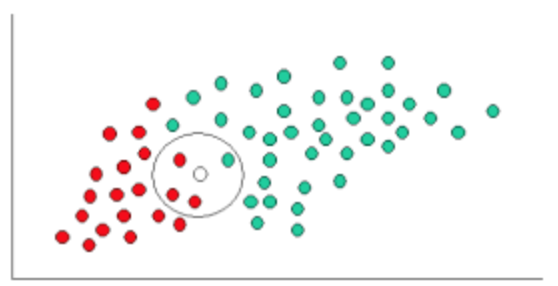
\includegraphics[width = 0.4\textwidth]{image.png}
\end{figure}


To demonstrate the concept of naive bayes classifcation consider the example illustrated in figure. 
The object depicted in the figure above belongs either the class green or red.  The task of the classifier is to classify new  observations and decide whether it belong to the class red or green. \\

Using bayes is this possible, first is the prior probability determined. In this case is it very likely to believe that a new obersevation would belong to the class green, since the amount green balls is larger than red.  The beliefs is known as the prior probability, is the probability based on prior experience. 

\begin{equation}
\centering
P(green) = \frac{number~of~green}{total~number~of~object}
\end{equation}

\begin{equation}
\centering
P(red) = \frac{number~of~red}{total~number~of~object}
\end{equation}

Using the prior probability, Will  a new object be classified. 

\begin{figure}[H]
\centering
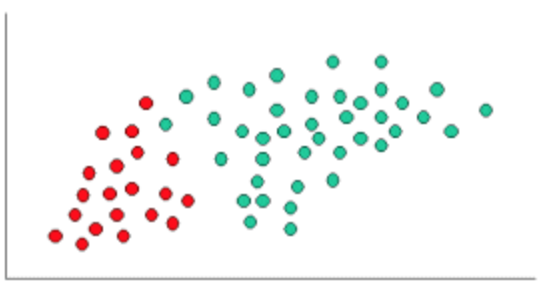
\includegraphics[width = 0.4\textwidth]{image2.png}
\end{figure}
The likelihood of the object either belonging to the class red or class green is completely determined by the object lying near it. 

\begin{equation}
\centering
likelihood~of~object~being~green = \frac{Number~of~green~in~the~vicinity~of~the~new~object }{total~number~of~green~object}
\end{equation}

\begin{equation}
\centering
likelihood~of~object~being~red = \frac{Number~of~red~in~the~vicinity~of~the~new~object }{total~number~of~red~object}
\end{equation}


In a bayesian analysis is the final classification produced by combining the prior and the likelihood information, to form the posterior probability, using the bayes rule . 


Formally can this be written as 
\begin{equation}
\centering
P(c|x) = \frac{P(x|c)P(c)}{P(x)}
\end{equation}

where 
\begin{itemize}
\item	$p(c|x)$ is the posterior probability of class given observation x
\item	$p(c)$ is the prior probability of class
\item   $p(x|c)$ is the likelihood which observation belongs to class  c
\item   $p(x)$ is the prior probability of the observation. 
\end{itemize}

\todo[inline]{https://documents.software.dell.com/statistics/textbook/naive-bayes-classifier}




 




\end{document}